\documentclass[../../Cours_M1.tex]{subfiles}

\newcommand{\nomTD}{TP3 : Asservissement numériques de position}
\renewcommand{\nomentete}{UE421 - \nomTD}
\renewcommand{\auteur}{A. Arnould, T. Colinot, C.Colonna}
\newcommand{\z}{z^{-1}}


\begin{document}

\titre{TP3 : Identification et asservissement numériques de position d'un bras à liaisons flexibles}

\section{Introduction}

On s'intéresse dans ce TP à la commande d'un montage disposant d'un bras entrainé par un moteur en liaison pivot élastique avec un chassis également en liaison pivot élastique avec le bâti.

\subsection*{Préparation 1}

\begin{itemize}
\item En utilisant la documentation fournie en annexe on trouve la constante de temps mécanique de la MCC  : $\tau_m = 17 ms$. On peut également déduire des valeurs de résistance et d'inductance fournie un ordre de grandeur de la constante de temps électrique de la machine : \[\tau_{el} = \frac{L}{R} \approx 80 \mu s << \tau_m\]

\item Comme la constante de temps mécanique est très grande devant la constante de temps électrique, on peut simplifier l'équation électrique donnée. \[u(t) = Ri(t) + \Phi\omega_m\]

\item En analysant les ordres de dérivation maximum atteignables par combinaison des équations électriques et mécaniques fournies, on trouve : \begin{itemize}
\item Pour $\theta$ : on arrive jusqu'à $\ddot{\ddot{\theta}}$, ce qui explique le degré 4 au dénominateur. Comme les expressions ne comportent que $\dot{\theta}$, on obtient un $(1-\z)$ en facteur.
\item Pour $\psi$ : on atteint $\dot{\ddot{\psi}}$, ce qui explique l'ordre 3 pour $V_\psi$.
\item Pour $U$ : on sait que le système est causal, ce qui impose les degrés des polynômes aux numérateurs.
\end{itemize}

\end{itemize}

\subsection*{Manipulation 1}

On injecte en entrée du système un créneau d'amplitude 2V crête-à-crête. On relève les signaux en sortie des capteurs de vitesse angulaire $\omega$ et de position angulaire du bras $\psi$. On obtient la courbe suivante :

\begin{figure}[h!]
\begin{center}
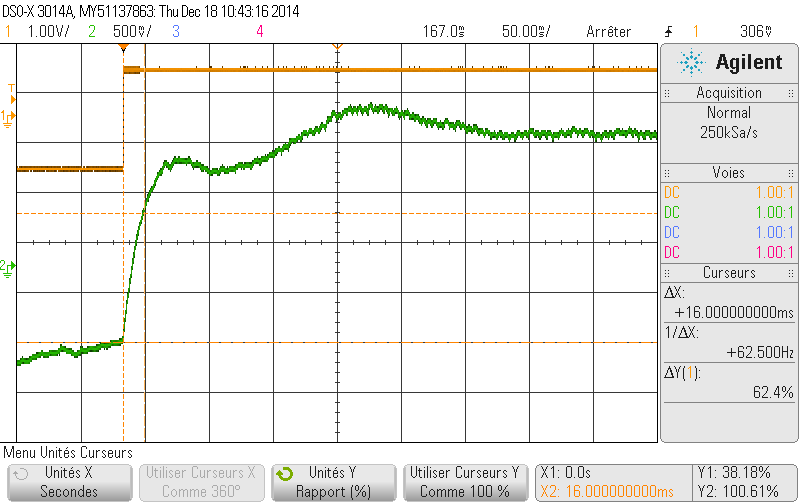
\includegraphics[width=0.7\textwidth]{tau.png}
\end{center}
\end{figure}

On relève le temps de montée du système approximé à un premier ordre, ce qui nous donne la bande passante du système. On trouve $\tau = 16 ms$ donc $F_max = 9.9Hz$. Une fréquence d'échantillonnage de 25ms est donc adaptée : elle conduit à une fréquence d'échantillonnage $F_e = 40Hz$ qui respecte la condition de Shannon : \[F_e > 2F_{max}\]

On peut approximer le système par un premier ordre, car la dérivée à l'origine de la réponse indicielle n'est pas nulle. Le comportement observé est donc uniquement dû à l'aspect mécanique du système. Cela prouve que la constante de temps électrique est négligeable, et justifie la simplification de l'équation électrique.

Pour une entrée sinusoïdale de fréquence 1Hz, on observe les angles $\theta$ et $\psi$ du système grâce à la carte Dspace et Simulink.

\begin{figure}
\begin{center}
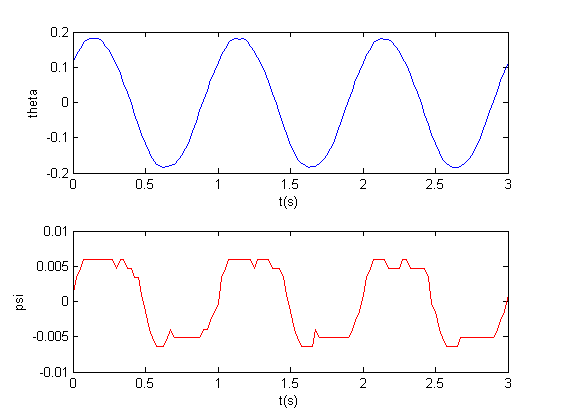
\includegraphics[width=0.7\textwidth]{CAN.png}
\end{center}
\end{figure}

\section{Identification}
\subsection*{Préparation 2}

\begin{itemize}

\item D'après l'équation (6) on trouve l'équation de récurrence : \[\gamma[k] + (a_1-1)\gamma[k-1] + (a_2-a_1)\gamma[k-2] + (a_3-a_2)\gamma[k-3] + (a_3-a_4)\gamma(k-4) = \Sigma_{i=1..4}b_iu[k-i]\]

\item On peut poser $\hat{\gamma}$ tel que $\hat{\gamma}[k] = \gamma[k] - \gamma[k-1]$.

\item On exprime $\hat{\gamma}[k]$ en fonction des termes précédents de $\hat{\gamma}$ et de $u$ :
\[\hat{\gamma}[k] = -\Sigma_{i=1..3}a_i\hat{\gamma}[k-i] + \Sigma_{i=1..4}b_iu[k-i]\]
d'où l'expression matricielle :
\[\hat{\gamma}[k] = \left[ -\hat{\gamma}_{k-1} \quad -\hat{\gamma}_{k-2} \quad -\hat{\gamma}_{k-3} \quad -\hat{\gamma}_{k-4} \quad u_{k-1} \quad u_{k-2} \quad u_{k-3}\right] \left[a_1 \quad a_2 \quad a_3 \quad b_1 \quad b_2 \quad b_3 \quad b_4\right]^{T} \]

\item D'après l'annexe 7 on obtient une expression de d[k] : \[d[k] = \left[-\hat{\gamma}[k-1] -\hat{\gamma}[k-2] ... -\hat{\gamma}[k-n] u[k-1] u[k-2] ... u[k-m]\right] \]
tel que $d[k]v = \hat{\gamma}\*[k,v]$

\item Par définition du SBPA, la grille fréquentielle est de $\frac{1}{NT_e}$. Pour $N=127$ et $T_e = 25ms$ on obtient 0.31Hz.

\end{itemize}

\subsection*{Manipulation 2}

On génère une séquence de bruit pseudo-aléatoire de longueur 7. On utilise pour ceci un registre à décalage, que l'on peut mettre en oeuvre sous Simulink comme suit :

\begin{figure}
\begin{center}
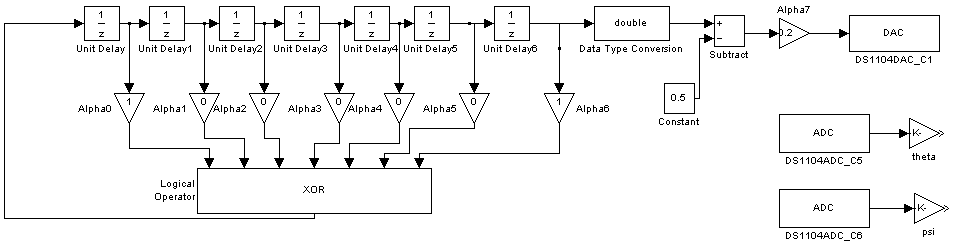
\includegraphics[width=0.7\textwidth]{SBPA.PNG}
\end{center}
\end{figure}

La transformée de Fourier du SBPA est :

\begin{figure}
\begin{center}
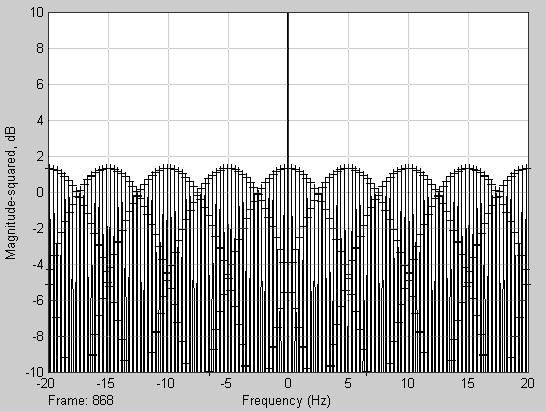
\includegraphics[width=0.5\textwidth]{spectroutroum.PNG}
\end{center}
\end{figure}

L'enveloppe de la densité spectrale de puissance a la forme d'un sinus cardinal périodisé. On vérifie que la grille fréquentielle est suffisamment fine pour caractériser le système.

On mesure les variations de l'angle du bras au cours du temps. On s'intéresse particulièrement au comportement fréquentiel de ce paramètre. La réponse en fréquence est donnée ci-dessous.


\begin{figure}[h!]
\begin{center}
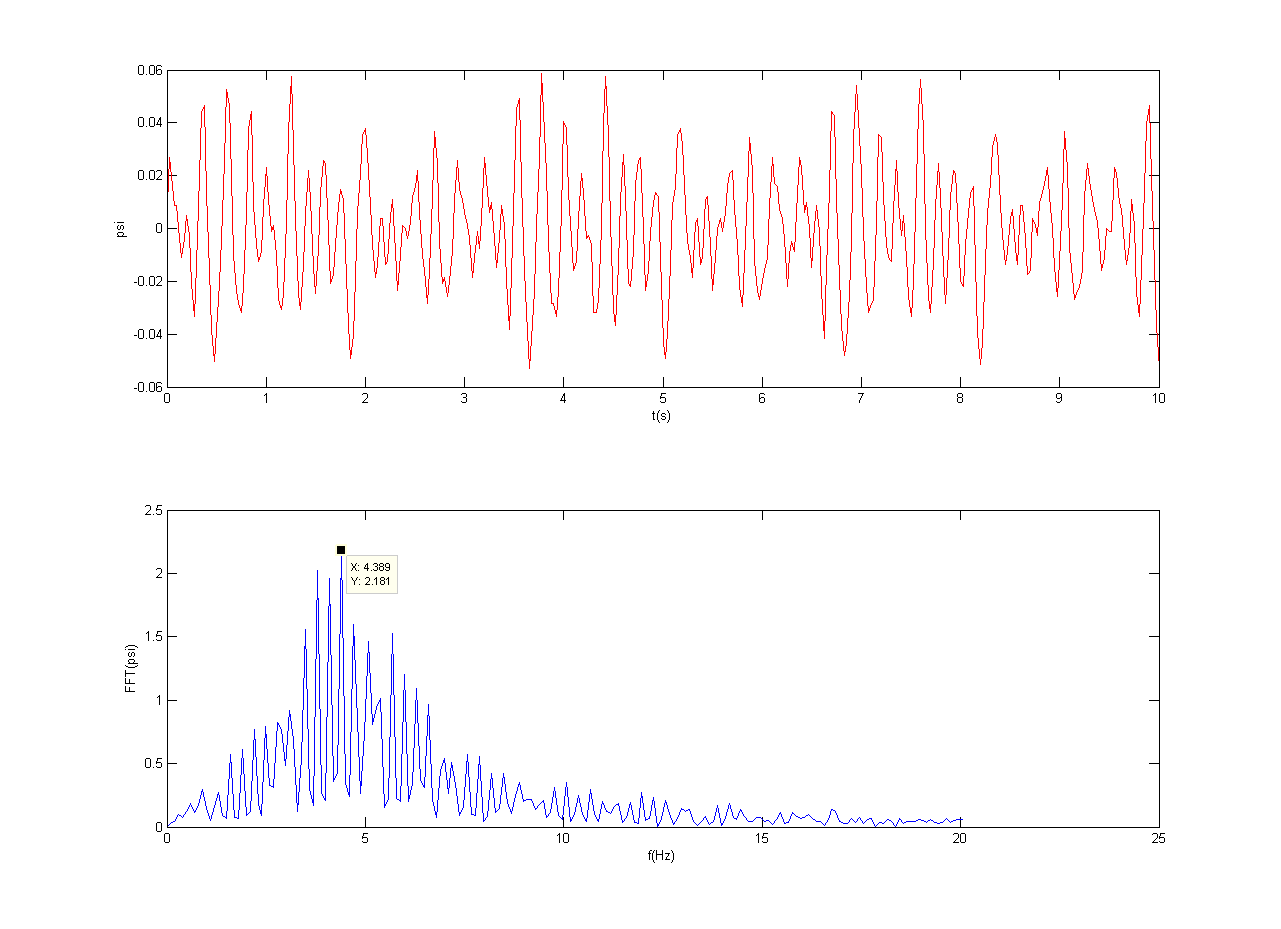
\includegraphics[width=0.5\textwidth]{FFTBG.png}
\end{center}
\end{figure}

Il existe des résonances matérialisées par des pics dans la réponse en fréquence. La plus importante se trouve à $F_{res} = 4.1Hz$. En excitant le système au GBF, avec un sinus de fréquence 4.1Hz, on remarque que cette résonance correspond à la fréquence où le bras oscille sans la plate-forme.

On veut identifier le système à partir de la forme choisie. Pour ce faire on met en oeuvre un critère des moindres carrés portant sur les paramètres du système. 

Le code matlab est donné ci-dessous :
\begin{lstlisting}
%kth=10/(2*pi);
%kpsi = 25/(2*pi);

mlibini

var_names={'Model Root/theta/Out1';'Model Root/psi/Out1';'Model Root/Alpha7/Out1'};
var=mlib('GetTrcVar',var_names);
mlib('Set','Trigger','off', 'TraceVars',var, 'StepSize',0.025, 'Start',0.0, 'Stop',5);

mlib('StartCapture');
while mlib('CaptureState')~=0,end
out_data=mlib('FetchData');
    
Te=0.025;
theta = out_data(1,:)-mean(out_data(1,:));
psi = out_data(2,:)-mean(out_data(2,:));
u = out_data(3,:)-mean(out_data(3,:));
gamma = psi+theta;


t=0:(length(out_data)-1);
t=t*Te;

hat_gamma = gamma - [0 gamma(1:end-1)];
hat_gamma_1 = [0 hat_gamma(:,1:end-1)];
hat_gamma_2 = [0 hat_gamma_1(:,1:end-1)];
hat_gamma_3 = [0 hat_gamma_2(:,1:end-1)];
hat_gamma_4 = [0 hat_gamma_3(:,1:end-1)];

u_1 = [0 u(:,1:end-1)];
u_2 = [0 u_1(:,1:end-1)];
u_3 = [0 u_2(:,1:end-1)];

d = [[-hat_gamma_1]; [-hat_gamma_2]; [-hat_gamma_3]; [-hat_gamma_4]; [u_1]; [u_2]; [u_3]];
d = d';
d = d(4:end,:);

v_opt = inv(d'*d)*d'*gamma(4:end)';

\end{lstlisting}

Les valeurs optimales sont \[v_{opt} = \vect{a_1 \\ a_2 \\ a_3 \\ a_4 \\ b_1 \\ b_2 \\ b_3} = \vect{-0,284 \\
-0,540 \\
-0,718 \\
-0,525 \\
-0,066 \\
0,007 \\
0,038}\]

\section{Asservissement de position}

\subsection*{Préparation 3}

\begin{itemize}

\item Le polynôme caractéristique monique s'exprime sous la forme \[\Pi_d(p) = 1+\frac{2m}{\omega_0}p + \frac{p^2}{w_0^2}
\]
Si on pose $p=\frac{1-z}{T_e}$ on trouve \[\Pi_d(z) = 1+\frac{2m}{\omega_0}\frac{1-z}{T_e} + \frac{(\frac{1-z}{T_e})^2}{w_0^2}\]
\[=1+\frac{2m}{\omega_0T_e}+\frac{1}{\omega_0^2T_e^2} + z(-\frac{2m}{ \omega_0T_e} - \frac{2}{\omega_0^2T_e^2}) + z^2(\frac{1}{\omega_0^2T_e^2})\]

\item Pour $e(z) = 0$ et $p(z) = cste$ on a \[lim_{n\rightarrow+\infty}(\epsilon[n]) = lim_{z\rightarrow1}(\epsilon(z)) = lim_{z\rightarrow1}(R(z)*(...))\]
donc si $R(z) = (z-1)\tilde{R}(z)$ on a bien : \[lim_{n\rightarrow+\infty}(\epsilon[n]) = 0\] ce qui correspond à une erreur statique nulle pour une perturbation constante.

\item L'équation diophantienne prend la forme : \[A(z)R(z) - B(z)R(z) = \Pi_d(z)A_0(z) \]
Par égalité des degrés : 

\item On prend $\omega = 100$.

\end{itemize}

\section*{Conclusion}

Si la forme de la fonction de transfert en z supposée est la bonne alors cette identification de système représente exactement la réalité.

On a utilisé un bruit blanc en entrée afin d'obtenir tous



\end{document}
